\documentclass{rapportECC}
\usepackage{lipsum}
\usepackage{amsmath} % Pour les environnements et commandes mathématiques avancées
\usepackage{amsfonts} % Pour les polices mathématiques supplémentaires
\usepackage{mathrsfs} % Pour les lettres script
\usepackage{hyperref} % Pour les hyperliens et les références croisées
\title{Rapport ECL - Template} %Titre du fichier
\usepackage{biblatex} %Imports biblatex package
\addbibresource{bibtex.bib} %Import the bibliography file
\usepackage{appendix} % Package pour gérer les annexes
\usepackage{ulem}
%
%%%%%%%%%%%%%%%%%%%%%%%%%%%%%%%%%%%%%%%%%%%%%%%%%%%%%%%%%%%%%%%%%%%%%%%%%%%%
\definecolor{peru}{RGB}{205,133,63}
\definecolor{DodgerBlue}{RGB}{30,144,255}
\definecolor{PAD}{rgb}{0.53, 0.15, 0.34}
\newcommand{\FAcom}[1]{\textcolor{peru}{~\textit{(\textbf{FL:}~{#1})}}}  % commentaires
\newcommand{\FAadd}[1]{\textcolor{DodgerBlue}{{#1}}}                     % ajouts/changements
\newcommand{\FAdel}[1]{\textcolor{DodgerBlue}{\sout{#1}}}                % suppressions 
%%%%%%%%%%%%%%%%%%%%%%%%%%%%%%%%%%%%%%%%%%%%%%%%%%%%%%%%%%%%%%%%%%%%%%%%%%%%
%
\begin{document}

%----------- Informations du rapport ---------

\titre{Les processus océaniques de sous-mésoéchelle} %Titre du fichier .pdf

\sujet{\LaTeX Approfondi} %Nom du sujet

\Encadrants{Francis \textsc{Auclair}
 \\Cyril \textsc{Nguyen} } %Nom de l'enseignant

\eleves{Naëla \textsc{Chehbouni}} %Nom des élèves

%----------- Initialisation -------------------
        
\fairemarges %Afficher les marges
\fairepagedegarde %Créer la page de garde
\tabledematieres %Créer la table de matières

%------------ Corps du rapport ----------------
\section{Introduction} 


\FAadd{Je dirais qu'il te faut commencer par une ou deux phrases introductives présentant le stage. Quel type de stage, dans quel type de cursus et dans quel environnement (labo, équipe...) ?}\\
Durant ce stage nous nous sommes intéressés à différents processus océanique de sous-mésoéchelle. \FAdel{Tentons de comprendre un petit peu ce qui ce cache derrière la notion de "sous-mésoéchelle".}
\FAadd{Évite au maximum le style "narration" dans un document scientifique. Certains éditeurs recommandent même de ne pas utiliser la première personne. Sans tomber dans l'excès, essaie d'épurer le style en adoptant une écriture précise et scientifique (chaque mot renvoie une notion clairement définie)...}

\subsection{Point sur les échelle  ou... L'océan et ses échelles caractéristiques...}
%regarder taylor thompson 2023
De façon générale lorsque nous présentons les différents phénomènes océaniques nous parlons de 3 échelles:\\
\FAadd{Le spectre des processus océaniques peut globalement être divisé en trois gammes d'échelles spatio-temporelles:}
\begin{itemize}
    \item la grande échelle : décrit la circulation globale de l'océan (circulation thermohaline...) \FAadd{ On parle aussi d'échelle synoptique}.
    \item la mésoéchelle : les transports d'Ekman, \FAadd{les courants géostrophiques et} les vents thermiques, \FAdel{les modèles de bassins, les modèles régionaux} \FAadd{A ce stade, ne mélange pas les échelles de processus et les modèles. Une fois les échelles dégagées, tu introduiras les modèles analytiques ou numériques.}.
    \item la microéchelle (comprenant aussi l'échelle moléculaire) : la turbulence \FAadd{homogène, isotrope et tridimensionnelle et sa cascade inertielle. Tu peux citer l'ouvrage de Frisch par exemple \cite{frisch_turbulence_1995}.}
\end{itemize}

Cependant, nous savons que la méso-échelle et la micro-échelle sont étroitement liées et échanges de l'énergie et de la vorticité. En effet, la petite échelle apporte de l'énergie à la grande échelle, tandis que celle-ci alimente la petite échelle en enstrophie (vorticité). Ces échanges se font par l'intermédiaire de processus de sous-mésoéchelle, on parle de "cascading". La difficulté est la suivante: où met-on les frontières de la sous-mésoéchelle ? \\ 

\FAadd{Pas exactement... A méso-échelle, on considère généralement que l'énergie cascade vers les grandes échelles alors que l'enstrophie, caractérisant la vorticité, cascade vers les plus petites échelles. On parle alors de \textit{cascade inverse} (vallis, 2006). Dans un tel modèle, la cascade turbulente à micro-échelle serait donc alimentée par les effets diabatiques dans les couches limites (friction, mélange...) or l'on sait aujourd'hui qu'une \textit{cascade directe} peut prendre naissance au sein même de la colonne d'eau, l'énergie étant alors au contraire transférée vers les plus fines échelles (taylor,2023). Le rôle joué par les processus de sous-mésoéchelle lors de la mise en place de cette cascade directe pose aujourd'hui encore de nombreuses questions (McWilliams, 2016).}

\FAdel{Regardons de plus près} quels sont les caractéristiques physiques qui pilotent les processus des différentes échelles. \FAdel{Au niveau de la mésoéchelle,}\\

Un critère potentiellement \FAadd{satisfaisant} \FAadd{pertinent} pour la frontière "supérieure" \FAadd{du spectre de sous-mésoéchelle} est le nombre de Rossby (la faut que je mette l'annexe avec les nombres principaux). La mésoéchelle se caractérise par un nombre de Rossby \FAdel{très} petit devant 1, on peut voir la transition vers la sous-mésoéchelle lorsque $Ro \approx 1$, \FAdel{c'est-à-dire lorsque la géostrophie devient de l'ordre de la vitesse horizontale du fluide.} \FAadd{i.e. lorsque les principaux "grands équilibres" (hydrostatique, géostrophie...) sont rompus.} \\
Là faut que je trouve un critère pour l'autre frontière + ref à McWilliams 2016

\begin{figure}[H]
    \centering
    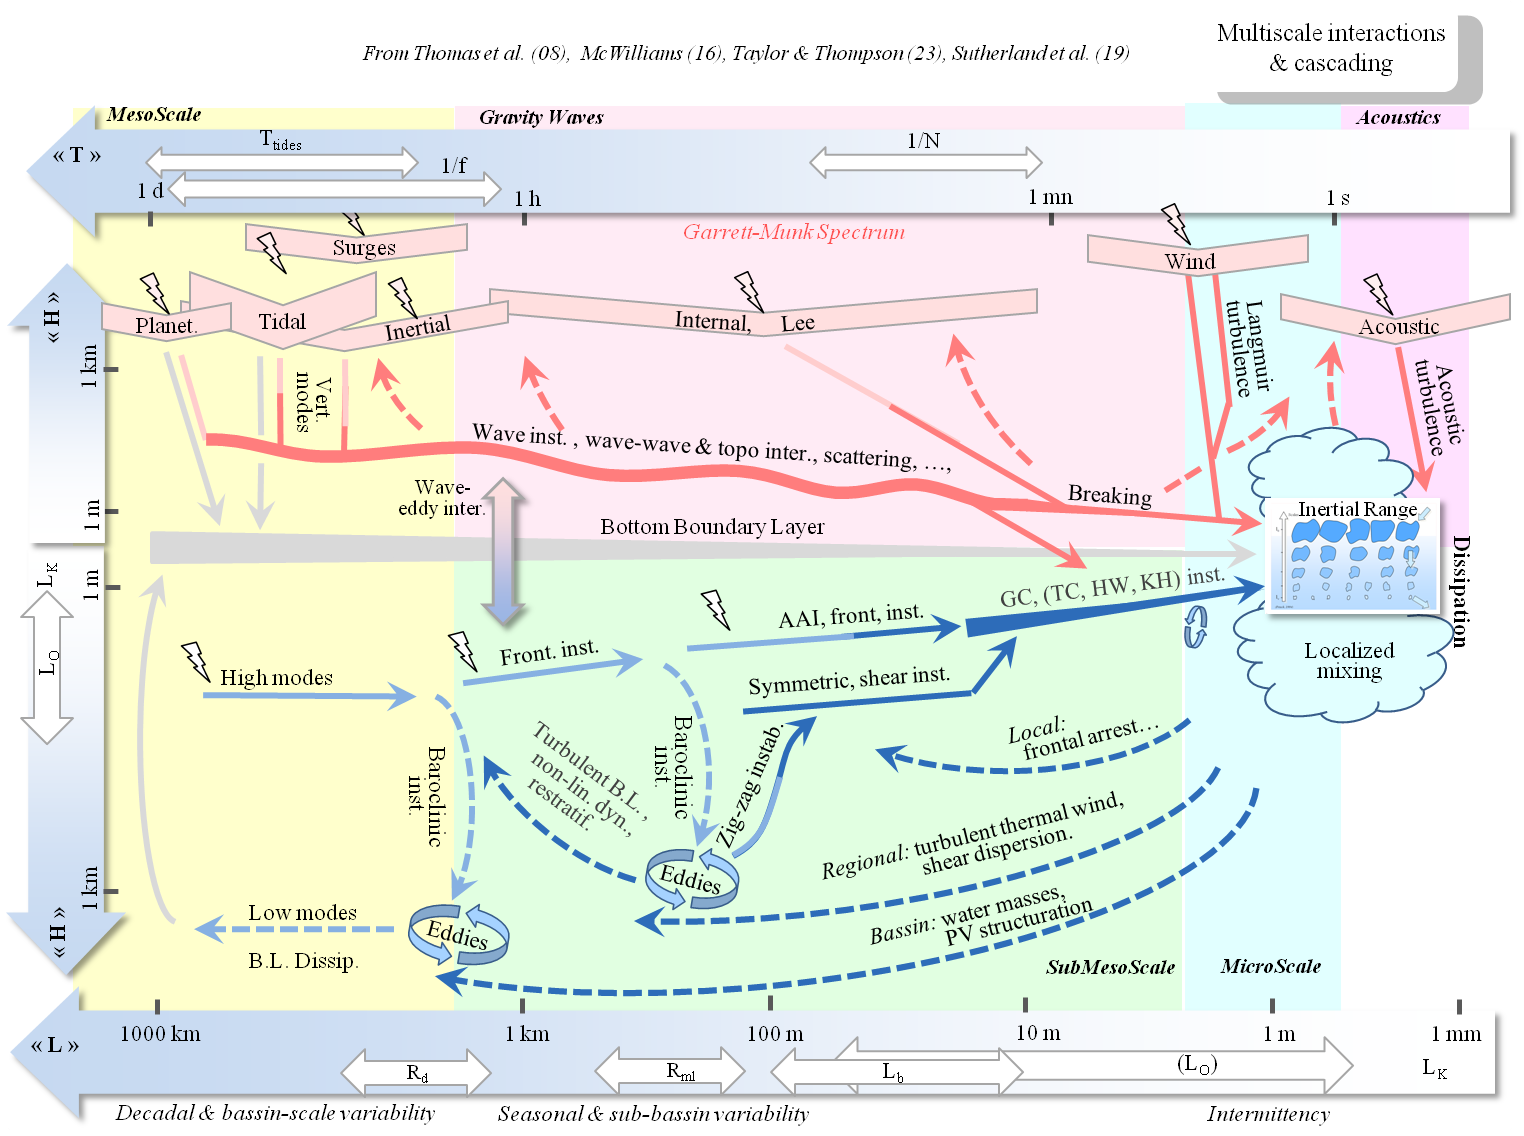
\includegraphics[width=1
    \textwidth]{images/sous_meso.png}
    \caption{Processus de sous-mésoéchelle et cascade d'énergie. \FAadd{Tu dois avoir une figure plus simple... Dans ta légende, tu dois donner un maximum d'informations pour faciliter la compréhension de la figure... Abscisses, ordonnées ? Couleurs ? Flèches ? etc...}}
    \label{fig:echelles}
\end{figure}

La figure \ref{fig:echelles} retrace les différents processus faisant le liens entre mésoéchelle, sous-mésoéchelle et microéchelle, dans l'océan et à la surface. Pendant ce stage, nous nous sommes plus spécifiquement intéressés à différents types \FAadd{de processus et d'instabilités de sous-mésoéchelle}: instabilités convectives, instabilités de cisaillement, mais aussi propagation des ondes acoustiques dans l'océan.
\\
Reste à savoir si je retravaille pas un peu l'image pour ne pas me perdre dans tout ça parce que y a beaucoup de chose. \FAadd{Oui, tout à fait, tu dois avoir une version beaucoup plus simple de cette figure. A la limite, tu peux ne pas la mettre...}

\subsection{Bases dynamiques des processus}
\label{Dynamiques globales}
L'ensemble de la dynamique des phénomènes étudiés s'appuie sur les équations de la mécanique des fluides et de la thermodynamique \FAdel{, ces 5 équations en particulier} :
\begin{equation}
    \frac{\partial \rho}{\partial t} = - \nabla \cdot (\rho \mathbf{v})
    \label{eq:continuite}
\end{equation}
\begin{center}
    \textit{Equation de continuité}
\end{center}
\begin{equation}
    \partial_t \rho \mathbf{v} = - \nabla (\rho \mathbf{v} \times \mathbf{v}) - 2\Omega \times \rho \mathbf{v} - \nabla p + \nabla (\mu (\nabla\mathbf{v} + \nabla\mathbf{v}^T) + \mu_2(\nabla \mathbf{v}) \mathbf{I}) +\rho \mathbf{g}
    \label{eq: qtt de mouvement}
\end{equation}
\begin{center}
    \textit{Quantité de mouvement, en densité}
\end{center}


\begin{equation}
    \partial_t \rho \theta = -\nabla(\rho\theta\mathbf{v}) + \nabla(\kappa_{\theta}\nabla\theta)
    \label{eq:chaleur}
\end{equation}
\begin{center}
    \textit{Equation de la chaleur}
\end{center}

\begin{equation}
    \partial_t \rho S = -\nabla(\rho S\mathbf{v}) + \nabla(\kappa_S\nabla S)
    \label{eq:salinite}
\end{equation}
\begin{center}
    \textit{Equation de la salinité} 
\end{center}
\begin{equation}
    \rho = \rho_{eos}(\theta , S, p)
    \label{eq:etat}
\end{equation}
\begin{center}
    \textit{Equation d'état}
\end{center}
\FAadd{Pour gagner de la place, utilise plutôt les "sous-équations" (regarde dans les documents que je t'ai donnés et mets sur la même ligne le type d'équation et sa formulation.}

\textit{Les termes des différentes équations  sont décrits sur l'Annexe 1.}
\\
\FAdel{On peut remarquer que l'équation \eqref{eq: qtt de mouvement} est écrite en terme de densité, ce choix est motivé par plusieurs raisons. Tout d'abord d'un point de vue physique, cette représentation permet de faire le lien avec les différents flux, à l'aide du théorème d'Ostrogradski. De plus, c'est également une méthode pour représenter numériquement les phénomènes, qui permet d'éviter certaines problèmes liés à la discrétisation.} \FAadd{Les équations du mouvement, de la chaleur et de la salinité (cite les labels... pour référence) sont données sous forme \textit{flux} afin de faciliter leur interprétation en termes de bilan, anticipant de plus leur formulation numérique.} \\

\vspace{0.5 cm}
\FAdel{La résolution de l'équation d'état \eqref{eq:etat} est très coûteuse numériquement parlant, c'est pour cela que dans le modèle Croco, qui sera présenté un peu plus tard nous avons privilégié une méthode de décomposition de la densité.} \FAadd{Afin de faciliter la résolution numérique de ce système, la dépendance de la densité en la pression totale peut être linéarisée (Auclair et al., 2024)...} En effet, on fait un développement limité autour de la pression hydrostatique $p_h$ :

\begin{equation}
    \rho_{eos}(\theta, S, p_h +\delta p) = \rho_{eos}(\theta, S, p_0) + c_s^{-2}(p_h - p_0) + c_s^{-2}\delta p
\end{equation}
\FAadd{A l'ordre 0 en anomalie de pression totale $(\delta p)$, il est encore possible de décomposer le profil de densité en une composante (statiquement) stable $(\rho_h)$ et une composante instable $(\rho_c)$. Il est à noter que cette décomposition n'est pas unique mais qu'elle est obtenue via un algorithme de montée/descente demandant un minimum de calculs (auclair et al., 2024):}
\begin{equation}
     \rho_{eos}(\theta, S, p_h +\delta p) =  \rho_h + \rho_c + c_s^{-2}\delta p
     \label{eq:decomp densite}
\end{equation}
\FAdel{Le développement au 1er ordre permet de linéariser la partie acoustique, ce qui revient moins cher numériquement.}
\vspace{0.5 cm}

\FAdel{Selon le cas que nous regardons, nous pouvons dégager des grandeurs caractéristiques qui permettent d'adimensionnaliser les équations de la mécanique des fluides.} \FAadd{Le modèle (référence) est toutefois très général et décrit une vaste gamme de processus dynamiques, il peut toutefois être simplifié en ciblant une gamme d'échelles caractéristiques et en adimentionnalisant chacunes des équations}. Ceci nous permettra de définir ce qu'on appelle des "régimes dynamiques", ce sont les nombres adimensionnels (Reynolds, Rossby etc...) qui nous donnerons des indications pour savoir dans quel régime nous nous trouvons.
, (les 4 derniers de la page du site wocean)
parler d'adimensionnalisation
\FAadd{Si tu choisis de présenter les régimes, tu peux effectivement ajouter en annexe les 4 derniers régimes. Tu dois alors les présenter et donnes leurs principales caractéristiques dans le texte en les rattachant aux 3 gammes d'échelles que tu viens de présenter.}

\section{Le modèle Croco}
Croco (Coastal and Regional Ocean COmmunity model) \FAadd{est un code communautaire d'océan régional, côtier ou encore littoral (hilt, 2020). Croco inclut des modules dynamiques, sédimentaires ou encore biogéochimique.} \FAdel{d'un point de vue dynamique, sédimentaire et biogéochimique avec une résolution spatiale allant du kilomètre au mètre. C'est un modèle communautaire, son développement vient donc des échanges entre différents laboratoires du monde.} \\


\subsection{Objectifs et hypothèses}
Au LAERO (Laboratoire d'Aérologie, Observatoire Midi-Pyrénées) l'équipe qui développe Croco se concentre sur la représentation dynamique et numérique des processus océaniques de sous-mésoéchelle. \FAadd{Cette équipe est plus spécifiquement en charge du noyau numérique non-hydrostatique et compressible en étroite collaboration avec l'équipe AIRSEA d'INRIA pour les aspects "calcul haute performances" (auclair 2024). }.\\
\FAadd{Si l'objectif demeure la simulation numérique réaliste de l'océan régional, les processus de sous-mésoéchelle sont toutefois systématiquement étudiés de façon isolée afin d'évaluer et faire évoluer l'ensemble des algorithmes et des schémas numériques. Des cas-tests académiques sont ainsi proposés et étudiés en détail d'un point de vue dynamique bien sûr mais aussi numérique et informatique ou HPC (voir par exemple l'étude des instabilités de cisaillement de type Kelvin-Helmholtz, centrales pour la mise en place de simulations LES\footnote{LES: Large Eddy Simulation, lorsque les grandes structures turbulentes menant à la cascade turbulente directe sont explicitement simulées.}: (Penney et al, 2020).}
\FAdel{sous la forme de cas-test}. On isole ainsi un processus et on essaie de le représenter de la façon la plus fidèle possible, en cherchant un compromis avec un amoindrissement des coûts \FAadd{de calcul et plus généralement des coûts environnementaux}. \\
Plusieurs hypothèses fondamentales ont été faites pour les représentations dynamiques, on parle notamment de représentation compressible et non-hydrostatique, deux hypothèses essentielles pour modéliser les ondes acoustiques. De plus, pour prendre en compte les ondes de surfaces, on considère l'existence d'un "toit libre", à l'inverse d'une surface océanique plate et rigide. \FAadd{Le choix de remettre en cause l'hypothèse de Boussinesq et de rendre le code compressible n'est pas dicté par la seule prise en compte des ondes acoustiques mais aussi par la nécessité de rendre le code \textit{non-hydrostatique} (auclair et al., 2018). En effet, sous l'hypothèse de Boussinesq, le calcul de la pression totale en écoulement non-hydrostatique requiert la résolution d'un système de Poisson tridimensionnel. La principale difficulté est dans ce cas liée au traitement de la surface libre et le choix fait dans le code Croco consiste à réintroduire les ondes acoustiques afin de conserver un système mathématiquement \textit{hyperbolique} et numériquement \textit{local} dans un contexte d'implémentation massivement parallèle.}



\subsection{Fonctionnement}
\FAadd{D'un point de vue plus informatique et en termes de calcul haute performance (dit HPC), le code océanique Croco est développé depuis le milieu des années 2010 par les équipes d'INRIA, du CNRS-INSU, d'IFREMER, du SHOM, de l'IRD et de l'Université de Toulouse III Paul Sabatier dans le cadre du Groupement de Recherche (GdR) éponyme. CROCO s'appuie à l'origine sur le code ROMS et plus spécifiquement ROMS-AGRIF choisi avant tout pour ses excellentes performances en termes de cout de calcul mais aussi de gestion de la mémoire (Shchepetkin \& McWilliams2005).}\\
Comme son parent ROMS, Croco repose sur certains principes de fonctionnements tel que le calcul parallèle s'appuyant sur la bibliothèque MPI: au lieu d'utiliser l'ensemble des processeurs à disposition pour faire les calculs sur une grille entière, le type de calcul parallèle \FAadd{choisi} permet de diviser la grille initiale \FAadd{en sous  domaines sur l'horizontale} et d'attribuer chaque \FAadd{sous-domaine} à un processeur qui échangera ensuite ses informations avec les autres processeurs. \\
Ensuite, concernant cette fois les coordonnées verticales, CROCO s'appuie sur une grille Arakawa-C et un système de coordonnées dites "s" \FAadd{qui suivent à la fois l'évolution de la bathymétrie et celle de la surface libre au cours du temps. \\
A l'image de sa version d'origine (hydrostatique), le noyau numérique compressible et non-hydrostatique de CROCO repose sur un traitement séparé mais couplé (\textit{time-splitting} en anglais) de la dynamique lente (géostrophie, courants d'Ekman...) et de la dynamique rapide, cette dernière concernant essentiellement la surface libre et la physique compressible et non-hydrostatique. Un schéma temporel prédicteur/correcteur original dit \textit{LFAM3 / Forward-Backward} est implémenté (Shchepetkin \& McWilliams2005 et auclair 2024).}\\

%%%%%%%%%%%%%%%%%%%%%%%%%%%%
systèmes de coordonnées verticales (terrain following "s")\\
grille c\\
systèmes à 2 pas de temps, "time splitting" \\
Schéma temporel time stepping (LFAM3-fb)\\

calcul parallèle MPI (message passing interface) (découpage sur l'horizontale) \\
architecture cpu(=calculateur classique) gpu(=graphic processing unit bco de processeurs mais moins performants)  à partir de open-acc (=standart de programmation pour ça), petites directives\\

%------------- Commandes utiles ----------------

\section{Les instabilités convectives}
\subsection{L'instabilité de Rayleigh-Taylor}

\FAadd{A l'instar de} l'instabilité de Rayleigh-Taylor, l'instabilité convective se déclenche à l'interface entre deux fluides de densités différentes, lorsque le fluide de densité forte est au-dessus du fluide de densité faible. \FAadd{La stratification est alors \FAadd{statiquement instable}.} \\ 
Regardons de plus près la description mathématique et numérique de ce processus.

\subsubsection{Analyse dynamique}

\FAdel{L'équation qui va beaucoup nous intéresser ici d'une part pour comprendre la dynamique du phénomène mais aussi pour proposer différentes représentations numériques est l'équation d'état \eqref{eq:etat}. }\\
\vspace{0.5 cm}
\FAadd{Au sein de la décomposition proposée en (référence de la relation), la composante $\rho_c$} est responsable du déclenchement de la convection. \FAdel{Cependant, on peut choisir une modélisation sans ce terme, ce qui reviendrait à considérer que l'instabilité vient du gradient de pression (voir \ref{sans rhoc}).} \FAadd{En l'absence de cette décomposition $(\rho_c=0)$,la convection peut toutefois être déclenchée de façon indirecte via l'action du gradient horizontal de pression hydrostatique puis de la composante compressible de ce même gradient de pression. Une question sous-jacente repose alors sur les conséquences dynamiques de ce choix numérique et l'on peut au final se demander si le mélange induite est in fine identique dans les deux cas.} \FAadd{Cette partie trouverait plus sa place dans la discussion des aspects numériques... Tu pourrais te contenter d'expliquer ce que sont les instabilités convectives et de RT...}

\\
\vspace{0.5 cm}
Le terme clé dans la compréhension du phénomène convection est la flottabilité. \\
On définit :
\begin{itemize}
    \item $\rho_0$ la densité de référence de Boussinesq
    \item $\rho_h$ la représentation du profil stable en densité
\end{itemize}
Dans ces conditions, on définit la flottabilité $b$ ainsi :
\begin{equation}
    b = \dfrac{-g}{\rho_0}(\rho_c - \rho_0)
\end{equation}
\FAadd{Si tu formules ce terme sans $\rho_0$ (il part quoiqu'il en soit avec le gradient vertical de pression), tu facilites grandement la discussion qui suit...}
\\
On voit donc le lien ici entre le mouvement vertical du fluide et la façon avec laquelle on décompose la densité. En effet la présence de :$\rho_c$ installe un régime de convection immédiat, car on aura $b \neq 0$. \FAadd{Pas avec la formulation actuelle!}\\

\subsubsection{Représensation numérique}

Le choix de cette décomposition de la densité est surtout lié à  des problématiques numériques, nous allons voir tout de suite les différences dans le processus de la convection selon la représentation que l'on choisit. \\
\FAadd{Une bonne pratique ici est de donner de façon rigoureuse l'ensemble des paramètres de la configuration que tu étudies, l'idée étant que ton lecteur doit être en mesure de la reproduire. Pour faire simple tu peux récupérer pour cela les "tables" écrites dans la papier en cours d'écriture que je t'ai passé: tu devrais y trouver tout ce dont tu as besoin. Pour les configurations acoustiques, tu devrais trouver l'équivalent dans le manuscrit de thèse de Pierre-Antoine.}
Dans les deux cas, on part du même état initial, on considère un fluide stratifié et stable dans lequel on plonge une goutte stratifiée avec deux densités différentes :

\begin{figure}[H]
    \centering
    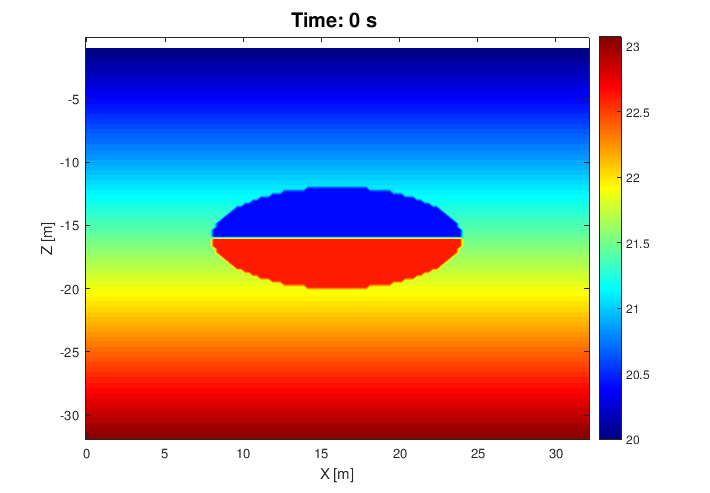
\includegraphics[width=0.7
    \textwidth]{images/Int_ConvT0.png}
    \caption{Instant initial \FAadd{Comme indiqué précédemment, tu dois détailler un peu ce qui est représenté: quelle variable, quelle type de section (verticale ici)... }}
\end{figure}


\vspace{1 cm}
\underline{\textbf{Avec le terme de convection :}}
\vspace{0.5 cm}

\\
Dans ce cas de figure le terme $\rho_h$ est calculé de sorte à  lisser le profil de densité pour en faire un profil stable (voir \§ à préciser). Dans le code, il est calculé au pas de temps lent. \\
Ainsi, dans cette première configuration $\rho_c$ représente l'anomalie autour du profil stable, il est calculé au pas de temps rapide. C'est donc ce terme qui déclenche la convection (cf équation (6)). \\

\begin{figure}[htb]
    \centering
    \subfloat[Etat du fluide au bout de 85 secondes]{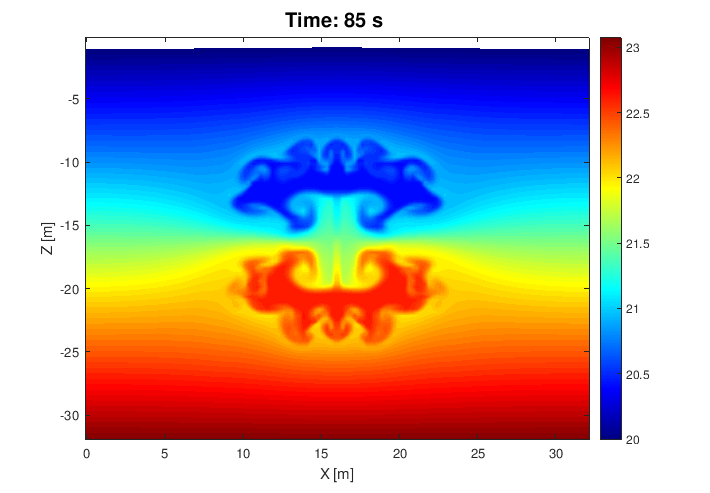
\includegraphics[width=0.45\textwidth]{images/avec_rhocS85.png}\label{fig:image1}}\hfill
    \subfloat[Etat du fluide au bout de 180 secondes. \\ Le mélange a débuté.]{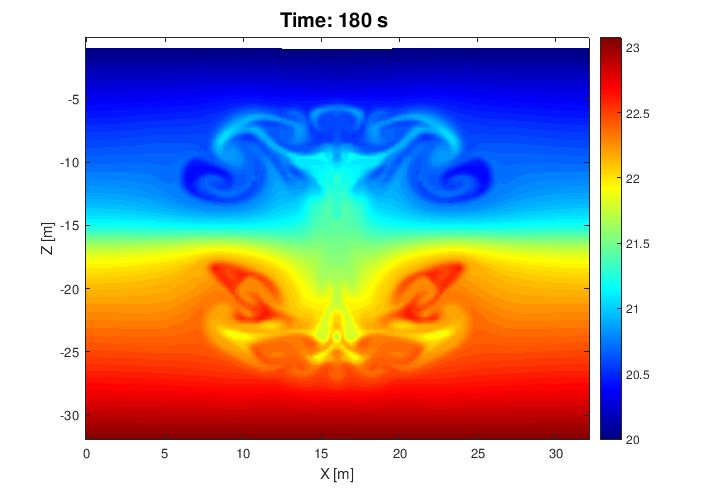
\includegraphics[width=0.45\textwidth]{images/avec_rhocS180.png}\label{fig:image2}}
    \caption{Description globale des deux images}
    \label{fig:images_cote_a_cote}
\end{figure}

Au bout de 85 secondes, nous arrivons à distinguer une sorte de flèche verticale \FAadd{(forme de champignon ?)}: c'est la forme caractéristique de l'instabilité de Rayleigh-Taylor. On remarque également des sortes de "vagues" autour de la flèche \FAadd{(structures se développant cette fois sur l'horizontale)}, ce sont des instabilités secondaires de Kelvin-Helmholtz, qui seront traitées plus tard (Cf \ref{KHI}).


\vspace{1 cm}


\underline{\textbf{Sans le terme de convection :}} 
\label{sans rhoc}
\vspace{0.5 cm}

\FAdel{Dans cette configuration là} Lorsque la décomposition de la densité ne fait pas apparaître le terme $\rho_c$, on a donc :
\begin{equation}
    \rho_{eos} = \rho_h + c_s^{-2}\delta p
\end{equation}
\FAdel{La convection vient d'abord du gradient de pression (cf équation (2)), d'où un mouvement plus porté par l'horizontale.} \FAadd{ L'action conjointe des composantes hydrostatiques et non-hydrostatiques du gradient de pression est à l'origine de forts cisaillements de courant le long de la surface externe de la bulle. En présence de stratification, des instabilités de cisaillement de type Kelvin-Helmholtz se déclenchent. Ces instabilités sont étudiées en détail par la suite (référence).}
\\
La simulation numérique donne :

\begin{figure}[H]
    \centering
    \subfloat[Etat du fluide au bout de 85 secondes]{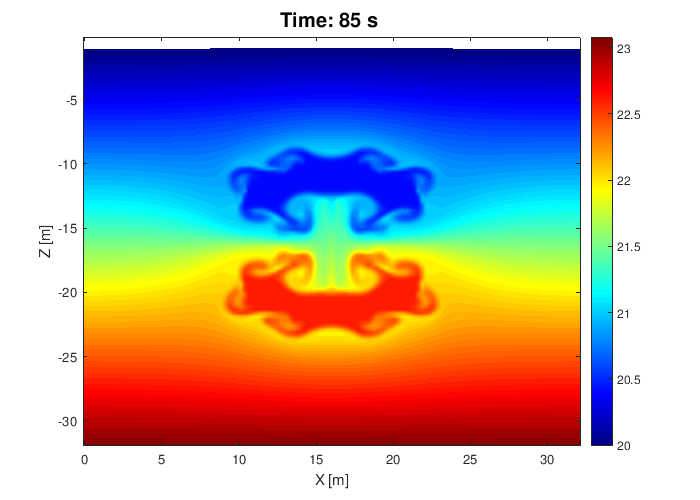
\includegraphics[width=0.45\textwidth]{images/sans_rhocS85.png}\label{fig:image1}}\hfill
    \subfloat[Etat du fluide au bout de 180 secondes. \\ Le mélange a débuté.]{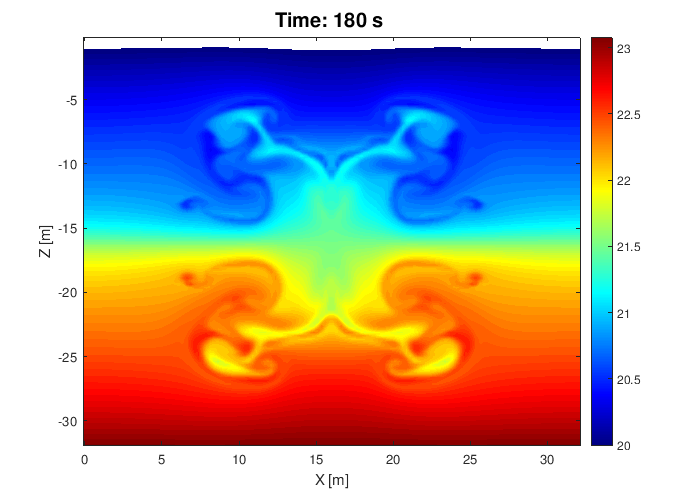
\includegraphics[width=0.45\textwidth]{images/sans_rhocS180.png}\label{fig:image2}}
    \caption{Description globale des deux images}
    \label{fig:images_cote_a_cote}
\end{figure}
\underline{\textbf{Conclusion partielle :}} \\
On remarque des différences dans le processus, notamment dans l'étendue verticale de la convection. On retrouve quand même les instabilités secondaires de Kelvin-Helmholtz, qui viennent du cisaillement des vitesses \FAdel{(elles-mêmes fruits du gradient de pression, cf \eqref{eq: qtt de mouvement}).}\\
On voit que le mouvement a une extension verticale beaucoup plus restreinte que lorsque la décomposition de $\rho$ prenait en compte $\rho_c$. \FAadd{Tu peux discuter aussi du fait que, même si tu ne le montre pas directement dans ton rapport, il a possible de montrer que l'état mélangé final n'est pas identique dans les deux cas... avant de conclure qu'il semble par conséquent important de représenter correctement le processus d'instabilité même si l'on est seulement intéressé par l'état final, i.e. une fois le mélange diapycnal terminé.}
\\
Parler de brunt vasiala

\subsection{L'instabilité de Kelvin-Helmholtz}
\label{KHI}
Là je comptais nommer les autres instabilités de cisaillements sans trop les détailler + parler un peu des ondes internes mais je sais pas à quel point c'est une bonne idée de parler de quelque chose sans le détailler.\\ \FAadd{Oui, ce serait parfait... Comme tu n'auras pas la place pour entrer dans les détails, tu devras aussi t'appuyer sur une ou plusieurs publications bien choisie(s).}
Cette instabilité se produit au niveau d'une interface de cisaillement de vitesse dans un fluide stratifié (c'est-à-dire, $N = cste$). \\

\subsubsection{Analyse dynamique}

On considère un fluide stratifié dans lequel on retrouve un cisaillement de vitesse. Plus précisément, sur la figure \ref{fig:KHI1} la partie bleue a une composante horizontale de vitesse égale à $-1 m \cdot s^{-1}$ \FAadd{(Ajoute des flèches indiquant la direction du courant directement sur la figure (a)}, tandis que celle de la partie rouge vaut $+1 m \cdot s^{-1}$. D'un point de vue statique, le fluide est stable, c'est-à-dire qu'on a $\rho_{bleu} < \rho_{rouge}$. \\
On exprime la vitesse du fluide sous la forme d'une anomalie autour du profil moyen U, on a donc $u = U+u'$ avec $u'<<U$. \\
On se place également sous l'hypothèse incompressible, ce qui nous permet d'écrire: 
\begin{equation}
    \mathbf{\nabla} \cdot \mathbf{u} = 0
\end{equation}
Ainsi, nous pouvons réécrire les équations de la mécaniques des fluides et de la thermodynamique (\ref{Dynamiques globales}) en fonction de $\psi$, la fonction de courant afin de réduire le nombre d'inconnues \FAadd{au prix d'une équation d'évolution présentant des dérivées partielles d'ordre plus élevé}. \FAadd{Pour homogénéiser les notations dans ton manuscrit, écris plutôt $\partial_{yy}U$.}
\\
On écrit :
\begin{equation}
    \psi(x,y,t) = \tilde{\psi}(y)exp(ik(x-ct))
    \label{eq: fct courant}
\end{equation}
Nous obtenons ainsi l'équation de Taylor-Goldstein : \\
\begin{equation}
    (U - c)(\tilde{\psi}_{zz} - k²\tilde{\psi}) + (\frac{N²}{U - c} - U_{zz})\tilde{\psi} = 0
    \label{eq: taylor goldstein}
\end{equation}

Comme écrit au début du paragraphe, d'un point de vue statique, le fluide est stable, il faut dont que l'instabilité soit \textbf{déclenchée}. \\

La stratégie adoptée pour mettre en évidence un critère de stabilité est la suivante : on rend $c$ complexe c'est à dire: $c = c_r + ic_i $. Ainsi, le système sera instable seulement si $c_i \neq 0$. Plus précisément, c'est le signe de $c_i$ qui nous indiquera la stabilité du système, le fait qu'il ne soit pas égal à 0 ne permet pas de le déterminer. Cependant, en retravaillant l'équation de Taylor-Goldstein \eqref{eq: taylor goldstein} et en supposant que $c_i \neq 0$, on obtient une condition nécessaire à remplir pour déclencher l'instabilité:
\begin{equation}
    N² - \frac{U_{z}²}{4} < 0
\end{equation}
En fait, cette condition a 2 solutions, une stable (pas de d'instabilité de Kelvin-Helmholtz donc) et une instable (celle qui nous intéresse), c'est pour cela qu'on qualifie cette condition de nécessaire non suffisante.\\
\FAdel{Ce qui donne :}\FAadd{Le critère nécessaire d'instabilité est donc:} $\frac{N²}{U_{z}²} < \frac{1}{4}$. 
Que l'on peut traduire par :

\begin{equation}
    Ri < \frac{1}{4}
\end{equation}


\subsubsection{Représentation numérique}
Le processus de mélange par instabilité de Kelvin-Helmholtz se déroule en plusieurs étapes. Tout d'abord après quelques instants \FAadd{(sois précise...)} à peine on distingue la phase \textbf{d'enroulement} (voir figure \ref{fig:KHI2}), la partie la plus dense du fluide s'enroule autour de la partie moins dense ce qui forme une sorte de vague. Ensuite, le "bout de la vague" s'étire donc, par conservation de matière, le fil s'amincit, c'est la phase \textbf{d'étirement} (figure \ref{fig:KHI3}). \FAadd{A ce stade, aucun processus diabatique n'est véritablement entré en jeu.} Jusque là, il n'y a pas de mélange, on voit encore bien les phases bleues et rouges du fluide, ce n'est qu'après la phase d'étirement que le mélange se fait (figure \ref{fig:KHI4}).
\begin{figure}[htbp] % L'argument [htbp] indique à LaTeX d'essayer de placer la figure "ici", "en haut de la page", "en bas de la page" ou "à la page suivante", selon ce qui convient le mieux.
    \centering
    \begin{minipage}{0.45\textwidth}
        \centering
        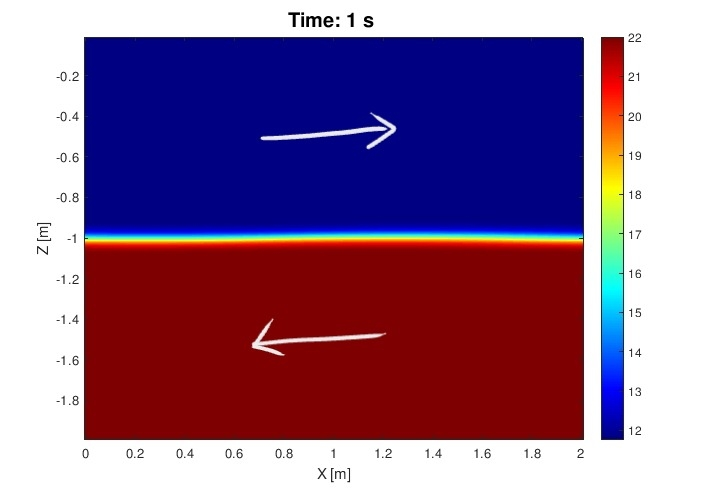
\includegraphics[width=\linewidth]{images/KHI1.png}
        \caption{Etat initial}
        \label{fig:KHI1}
    \end{minipage}
    \hspace{0.05\textwidth} % Espace horizontal entre les deux images
    \begin{minipage}{0.45\textwidth}
        \centering
        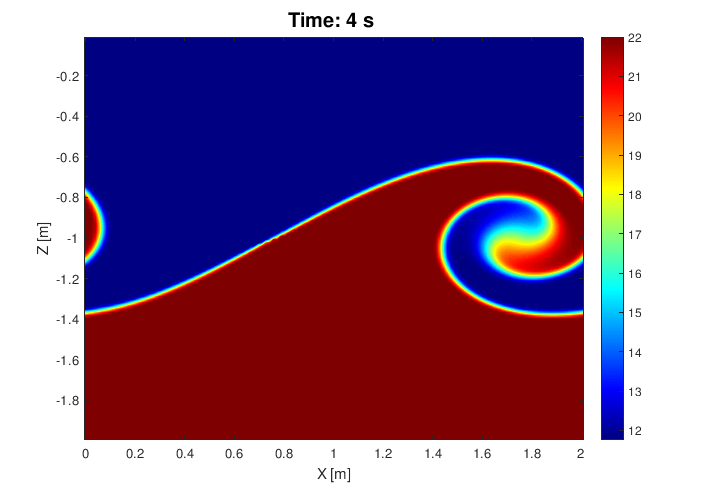
\includegraphics[width=\linewidth]{images/KHI2.png}
        \caption{Phase d'enroulement}
        \label{fig:KHI2}
    \end{minipage}
    \begin{minipage}{0.45\textwidth}
        \centering
        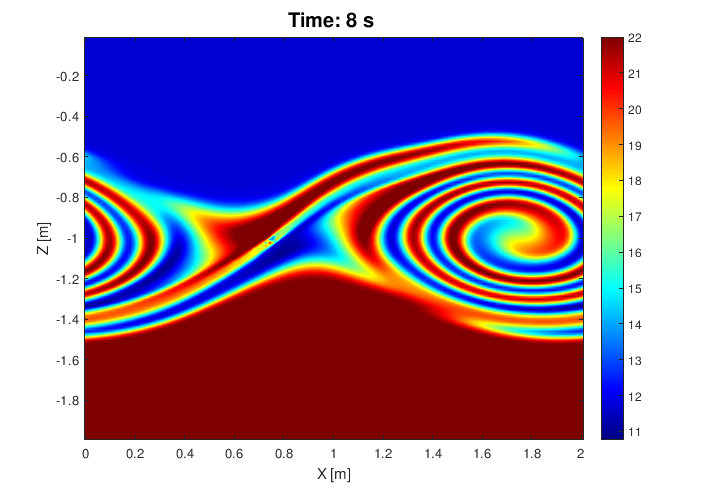
\includegraphics[width=\linewidth]{images/KHI3.png}
        \caption{Phase de brassage}
        \label{fig:KHI3}
    \end{minipage}
    \hspace{0.05\textwidth} % Espace horizontal entre les deux images
    \begin{minipage}{0.45\textwidth}
        \centering
        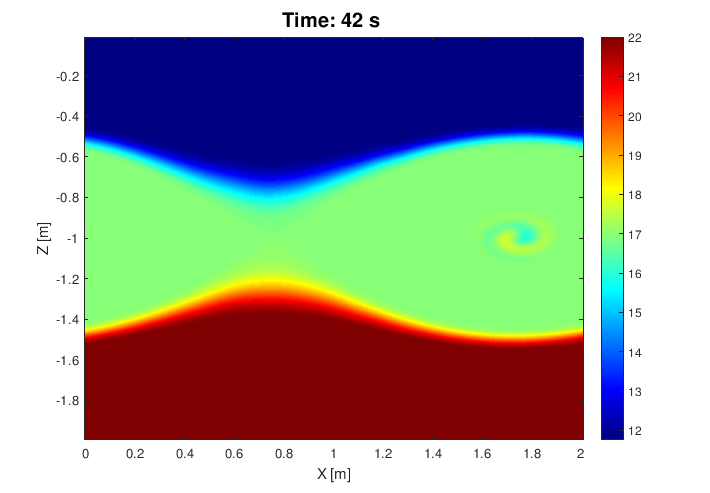
\includegraphics[width=\linewidth]{images/KHI4.png}
        \caption{Mélange}
        \label{fig:KHI4}
    \end{minipage}
\end{figure}

\FAadd{Petites conclusion partielle: quels étaient les objectifs et quels sont tes conclusions ? Comme pour la section précédente, tu peux dire que la représentation de l'instabilité est correcte et qu'il a par ailleurs était possible de montrer que le déclenchement (numérique) respecte bien le critère nécessaire. Tu as le résultat dans le papier que je t'ai donné... on montre de plus que la croissance initiale de l'instabilité numérique est tout à fait similaire à ce que donne une analyse de stabilité linéaire. Enfin tu peux plus généralement citer le papier de Jared Penney dans lequel le mélange des traceurs est plus spécifiquement étudié. A toi de voir par contre ce que tu souhaites garder pour la conclusion partielle et pour ta discussion finale.}\\






\section{Les ondes acoustiques: propagation en océan stratifié}

Nous allons maintenant nous intéresser à la propagation des ondes acoustiques dans l'océan. Cela peut avoir des applications intéressantes notamment dans la prévention des risques \FAadd{lors de la génération d'évènements potentiellement catastrophiques tels que les tsunamis}. Effectivement, les ondes acoustiques \FAadd{générées lors de la mise en mouvement initiale de la colonne d'eau par les forçages du tsunami,} se déplacent dans l'océan à une vitesse d'environ 1 500 $m \cdot s^{-1}$, à titre de comparaison les vagues d'un tsunami peuvent aller à 300 $m \cdot s^{-1}$. Ainsi, trouver une caractérisation acoustique de ces phénomènes pourrait améliorer leur détection et donc dans ce cas précis anticiper l'évacuation de la population.

\subsection{Postulats dynamiques}
\subsubsection{Mise en équation}


On part des équations habituelles de la mécanique des fluides et de la thermodynamique\FAadd{pars plutôt de ton système initial que tu peux citer)} . (phrase sur le régime) \FAadd{Oui, ce serait parfait, tu peux d'ailleurs faire de même pour les deux instabilités étudiées précédemment.}
\\
On néglige la force de Coriolis, la viscosité et le coefficient de diffusivité. \FAadd{Tu peux préciser que l'on conserve par contre la seconde viscosité (moléculaire) liée à la dissipation de l'onde acoustique et ce en particulier dans le sédiment.}
\\
Ce n'est pas une équation de d'Alembert classique que vérifie la pression ici, en effet il faut prendre en compte la vitesse et la non-homogénéité du fluide. Voici l'équation que propose Godin[2011] cf thèse PAD \FAadd{Cite la thèse après l'avoir référencée.}
\begin{equation}
    \frac{d}{dt}[\frac{d}{dt}(\frac{1}{\rho c²}\frac{dp}{dt}) - \nabla \cdot \frac{\nabla p}{\rho}] + 2\frac{\partial \mathbf{u}}{\partial x_i} \cdot \nabla (\frac{1}{\rho}\frac{\partial \rho}{\partial x_i}) = 0
\end{equation}

Cependant, cette équation ne retranscrit \FAdel{pas vraiment} \FAadd{ qu'une partie de} ce qu'on cherche à représenter. En effet, nous souhaiterions prendre en compte les conditions aux limites: les sédiments au fond de l'océan et à la surface libre, car celles-ci sont essentielles pour comprendre le concept de propagation en modes. cf OM2021

\subsubsection{Concept de modes de propagation}

A la manière de la propagation d'une onde électromagnétique dans une fibre optique \FAadd{(référence?)}, l'onde acoustique ici se réfléchit à la fois à la surface et au fond de l'océan. Cela conduit notamment à des interférences entre les différents fronts réfléchis. Les interférences constructrices forment ce qu'on appelle des "modes de propagation". On numérote également ces modes: les numéros correspondent au nombre de réflexion avant l'interférence. On comprend donc que plus le mode est élevé, moins le front est rapide. \\
Là il me manque une image mais j'en trouve pas de satisfaisante, je la créerai peut etre moi même. \FAadd{ Cite et reprend l'ouvrage de Jensen (je pense te l'avoir donné en pdf... il est assez pédagogique (à mon goût en tout cas) et contient de nombreuses illustrations.}
%c dans un milieu non borné
\\

Décrire avec un article OM2021 pour les conditions aux limites
autre publi: revisiting oceaninic acoustic gravity surface waves
\FAadd{L'idée de ces publications est de proposer une modèle de dispersion à 2 équations suffisamment général pour englober ondes acoustiques, ondes de gravité interne et ondes de gravité de surface dans un océan stratifié et compressible. Tu peux en profiter pour souligner une certaine ressemblance entre modes acoustiques et modes gravitaires internes. }

\subsection{Popagation en 2d dans un océan stratifié en prenant en compte la bathymétrie}


\subsubsection{Cas général avec une bathymétrie marquée}

\begin{figure}[H] % L'argument [htbp] indique à LaTeX d'essayer de placer la figure "ici", "en haut de la page", "en bas de la page" ou "à la page suivante", selon ce qui convient le mieux.
    \centering
    \begin{minipage}{0.45\textwidth}
        \centering
        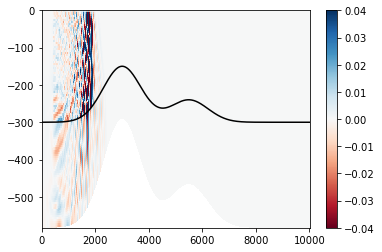
\includegraphics[width=\linewidth]{images/im2.png}
        \caption{Image 1}
        \label{fig:image1}
    \end{minipage}
    \hspace{0.05\textwidth} % Espace horizontal entre les deux images
    \begin{minipage}{0.45\textwidth}
        \centering
        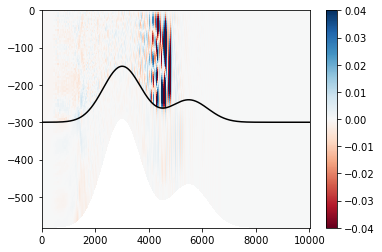
\includegraphics[width=\linewidth]{images/im4.png}
        \caption{Image 2}
        \label{fig:image2}
    \end{minipage}
    \vspace{1cm} % Espace vertical entre la première ligne et la deuxième image
    \begin{minipage}{0.9\textwidth}
        \centering
        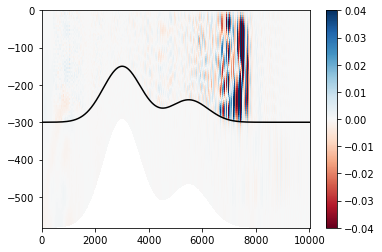
\includegraphics[width=0.45\textwidth]{images/im6.png}
        \caption{Image 3}
        \label{fig:image3}
    \end{minipage}
    \caption{Description générale des images.}
    \label{fig:three_images}
\end{figure}
Pour la première configuration, on considère une onde acoustique émise à 100 mètres de profondeur, dans un environnement avec une bathymétrie marquée. \\
Les "taches" que l'on voit sur les figures représentent les modes de propagation. \\
D'ailleurs, à  partir de la deuxième image on voit bien que l'onde \FAdel{a l'air de se propager}  \FAadd{se propage} plus vite dans le sédiment que dans l'océan, on aperçoit également la réfraction de l'onde dans le sédiment qui retourne dans l'océan, qui se trouve donc devant le front d'onde.\\
On remarque également l'atténuation de l'onde dans le sédiment, bien qu'elle se déplace plus vite dedans.

\\
\vspace{1 cm}

Ensuite, nous avons refait des simulations en changeant à la fois la nature du sédiment (argile ou sable) mais aussi la profondeur de l'océan (150 et 300 mètres)
\subsubsection{Influence du sédiment}
On  compare la propagation d'une onde acoustique dans un océan de 150 mètres de profondeur en fonction de la nature du sédiment. \\
Pour l'argile, on a pris une vitesse de compression de $1550 m \cdot s^{-1}$ et une densité égale à $1.7 kg \cdot dm^{-3}$ .
\\
Pour l'agile, on a pris une vitesse de compression de $1800 m \cdot s^{-1}$ et une densité égale à $2 kg \cdot dm^{-3}$. \FAadd{Deux fois la même phrase ? Je ne suis pas sûr de bien suivre ?}\\
D'ailleurs la vitesse de compression dans un sédiment dépend entre autre de sa densité, plus le milieu est dense, plus l'onde se propage rapidement.
\begin{figure}[H]
    \centering
    \subfloat[Propagation dans un milieu argileux]{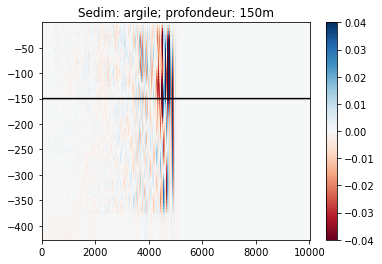
\includegraphics[width=0.45\textwidth]{images/im4_150_argile.png}}\label{fig:image1}\hfill
    \subfloat[Propagation dans un milieu sableux]{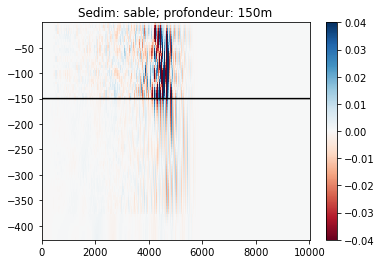
\includegraphics[width=0.45\textwidth]{images/im4_150_sable.png}\label{fig:image2}}
    \caption{Influence du sédiment dans la propagation d'une onde acoustique}
    \label{fig:images_cote_a_cote}
\end{figure}
Ainsi, comme on pouvait s'y attendre, l'onde se déplace plus vite dans le sable que dans l'argile. Cependant, il semblerait que le sable soit un milieu plus dispersif que l'argile dans la mesure où l'onde à l'air de s'atténuer beaucoup plus rapidement dans le milieu sableux.

\subsubsection{Influence de la profondeur}

Maintenant comparons la propagation de l'onde dans un même milieu mais pour des profondeurs différentes. 

\begin{figure}[H]
    \centering
    \subfloat[Propagation dans un océan de 150 mètres de profondeur]{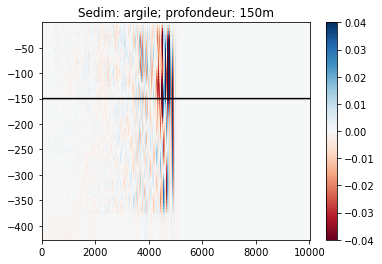
\includegraphics[width=0.45\textwidth]{images/im4_150_argile.png}}\label{fig:image1}\hfill
    \subfloat[Propagation dans un océan de 300 mètres de profondeur]{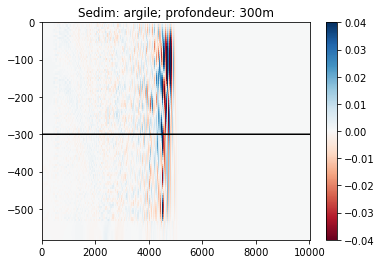
\includegraphics[width=0.45\textwidth]{images/im4_300_argile.png}\label{fig:image2}}
    \caption{Influence de la profondeur dans la propagation d'une onde acoustique}
    \label{fig:images_cote_a_cote}
\end{figure}
Dans l'océan profond de 150 mètres, l'onde semble complètement atténuée vers une profondeur de -370 mètres. Pour celui profond de 300 mètres, l'onde résiste au delà de 500 mètres de profondeur. Globalement dans les deux océans les ondes sont atténuée dans le sédiment après une distance caractéristique autour des 200 mètres. 
\vspace{1 cm}
Finalement, on comprend que plusieurs facteurs rentrent en jeu lorsqu'il s'agit d'évaluer la propagation d'une onde acoustique dans l'océan. Tout d'abord la profondeur des eaux joue sur la distance maximale que l'onde pourra atteindre avant d'être atténuée. D'autre part, la nature du sédiment influence la vitesse de propagation de l'onde, en effet l'onde se propage plus vite dans le sable, c'est-à-dire dans le milieu le plus dense (la masse volumique du sédiment n'est pas le seul paramètre à prendre en compte).\\
\FAadd{Petit conclusion partielle ici aussi... Tu peux d'ailleurs reprendre le paragraphe précédent. Prends juste un peu de recule: que t'apporte cette partie de l'étude ?}
\section{Discussion et conclusion}

\FAadd{Nous avions commencé en discuter, tu peux rédiger 2-3 parties:
\begin{itemize}
    \item Discussion des résultats scientifiques: résume de façons très synthétiques tes résultats sur ton choix de processus de sous-mésoéchelle.
    \item Conclusion scientifique: tu as souligné en introduction l'importance du spectre de sous-mésoéchelle... En quoi ton étude permet-elle d'avancer ? Tu peux par exemple discuter du fait que cette étude ciblant les processus permet de mieux comprendre la dynamique spécifique de chaque processus bien sûr mais aussi d'évaluer la pertinence du protocole de modélisation numérique avec CROCO: aspects numériques et HPC.
    \item Perspectives scientifiques: tu peux par exemple discuter du fait qu'une petite partie seulement du chemin est faite avec ces études académiques... L'océan étant très non-linéaires, la somme des processus ne permets malheureusement pas de conclure sur la qualité de la prévision!
    \item A toi de voir, mais je pense qu'il te faut rédiger un petit paragraphe pour la conclusion du stage à proprement parlé en reprenant les objectifs fixés par l'ENS.
    
\end{itemize}}

\newpage


\printbibliography


% Ajout de l'annexe
\newpage
\begin{appendices}
\section{Annexe : }
Dans cette section de l'annexe, nous fournissons des détails supplémentaires.
\subsection{Définition des variables}
%%%%%%%%%%%%%%%%%%%%%%%%%%%%%
%%% Tableau des variables %%%
%%%%%%%%%%%%%%%%%%%%%%%%%%%%%
{\renewcommand{\arraystretch}{1.5}
\begin{table}
\begin{center}
\begin{tabular}{ l l }
\hline 
$\mathbf{g} = (0,0,g)$ &  accélération de la pesanteur \\
$\boldsymbol{\Omega} = (0,f^\perp/2,f/2)$ & vecteur de vitesse angulaire dans le référentiel local \\
%$\boldsymbol{\tau}$  & viscous stress tensor \\ 
$\nabla = (\partial_x, \partial_y, \partial_z)$ & opérateur gradient en coordonnées cartésiennes\\
$\mathbf{x} = (x,y,z)= (x,y,\mathscr{s})$ & spatial location in Cartesian and $\mathscr{s}$-coordinates\\
$\mathbf{\nabla}_{\mathscr{s}}.(\rho h \mathbf{v})= \partial_{x} \rho h u \big\vert_\mathscr{s}+\partial_\mathscr{s}\rho v_\mathscr{s}$ & Advection in flux form and $\mathscr{s}$-coordinates \ref{Eq_mass_s} \\
\hline
$\mathbf{v} = (u,v,w)$, $\mathbf{u} = (u,v,0)$  & 3D, horizontal velocity vector  \\ 
$(\theta,\rho,S)$ & Potential temperature and density and salinity \\
$\zeta(x,y,t)$ & free-surface elevation \\
$\psi$ & any physical intensive, specific, scalar variable. \\
$\rho_0$  &  Boussinesq reference density \\
$p_0(z) = - \rho_0 g z$ & background hydrostatic pressure   \\
$p_{\rm h}=-\rho_{\rm h} g$  & hydrostatic pressure based on the statically-stable portion of the density field\\
$\rho_{\rm c} = \rho_{\rm eos}(\theta,S,p_0)-\rho_h$  & statically-unstable portion of the density field \\
$\delta p=c_s^2\delta\rho$  & compressible pressure and density anomalies with $c_s$ the speed of sound \\
\hline
$\mu$ ($\mu_2$)  & dynamic (bulk or second) viscosity  \\
$\kappa_\theta$ ($\kappa_S$) & thermal (salt) diffusivity\\
\hline 
\end{tabular}
\end{center}
\caption{\textit{summary of the main notations.}}
\label{Table_notations}
\end{table}
}
%%%%%%%%%%%%%%%%%%%%%%%%%%%%%
%%% Tableau des variables %%%
%%%%%%%%%%%%%%%%%%%%%%%%%%%%%
Vu que j'ai récupéré ce tableau dans "Papier Croco" qui est pas encore sorti, je peux le citer ou pas ?

\end{appendices}

\end{document}
